\documentclass[11pt]{article}
\usepackage{latexsym}
\usepackage{amsmath}
\usepackage{graphicx}
\DeclareGraphicsExtensions{.pdf,.png,.jpg}
\usepackage[top=1in, bottom=1in, left=1in, right=1in]{geometry}

\parindent0pt
\parskip\bigskipamount

\usepackage{colortbl}
\usepackage{pgfplots}
\usepackage{pgfplotstable}



\begin{document}
		\begin{figure}
	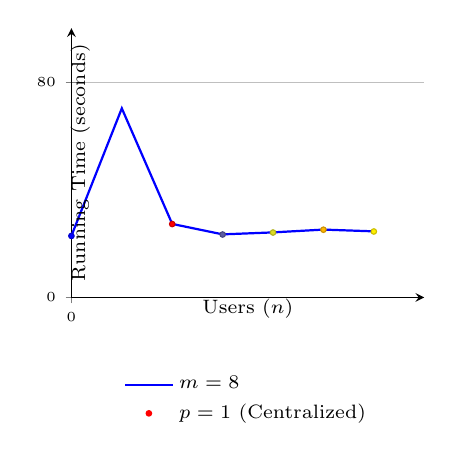
\begin{tikzpicture}
	\begin{axis}[
		width=0.5\linewidth,
		height=5cm,
		axis lines=left,
		grid=both,
		legend style={draw=none, font=\scriptsize},
		legend cell align=left,
		legend style={at={(0.5,-0.25)}, anchor=north},
		label style={font=\scriptsize},
		ticklabel style={font=\tiny},
		xlabel style={at={(0.5, 0.03)}},
		ylabel style={at={(0.08, 0.5)}},
		ymin=0,
		xmin=0,
		ymax=100,
		xmax=7,
		xtick={0,10},
		ytick={0,80},
		xlabel=Users ($n$),
		ylabel=Running Time (seconds),
		legend entries={{$m=8$, $p=1$ (Centralized)}},
		]
		\addplot[color=blue, thick, mark options={scale=0.5}] coordinates {
		(0, 22.87835501)
		(1, 70.22758985)
		(2, 27.29357997)
		(3, 23.41346661)
		(4, 24.14684022)
		(5, 25.18932616)
		(6, 24.53572075) };
		\addplot[scatter,color=red, only marks,mark=*, mark options={scale=0.5}] coordinates {
		(0, 22.82923962950044)
		(2, 27.246690713625878)
		(3, 23.363384835018515)
		(4, 24.096623164811717)
		(5, 25.14073766356739)
		(6, 24.486286272271638)};
	%	\addplot[color=black!40!green, mark=diamond*, thick, mark options={scale=0.5}, dashed] coordinates {
		%	(25, 1) (50, 1) (75, 10) (100, 35) (125, 140) };
	\end{axis}
\end{tikzpicture}
		\caption{\scriptsize Performance comparison of the algorithms ($m=30$)} \label{fig:label9}	
	\end{figure}
	
\centering\large \textbf{[ Robust Optimization ]}
	
	\begin{align*}
	\text{(Original)} \quad \min  \quad & d^T\Omega d  - \lambda d^T \alpha 
	\end{align*}
	\\
	Let set $U := \{ \tilde \alpha  \mid \tilde \alpha_i = \hat{\alpha_i} + \bar{\alpha_i}\gamma_i , \quad -1 \leq \gamma_i\leq 1 , \quad \sum_{i} |\gamma_i| = \Gamma \}$.
	\\
	
	
	\begin{align*}
	\text{(robustness)} \quad \min \quad & d^T\Omega d  - \lambda \min_{\tilde \alpha \in U } d^T \tilde{\alpha} \\
	\text{$\Rightarrow$} \quad \min_{\tilde \alpha \in U } d^T \tilde{\alpha} &= \min \sum_{i} d^T (\hat{\alpha_i} + \bar{\alpha_i}\gamma_i ) \\
	\text{(Dual) $\Rightarrow$} \quad \max \quad & \Gamma \pi + \sum_{i} \theta_i  \\
	\text{s.t} \quad & \pi + \theta_i \leq   \bar{\alpha} d_i, \quad \forall i \in N \\
	& \pi \geq 0, \quad \\
	&  \theta_i \geq 0, \quad \forall i \in N 
	\end{align*}
	
	
	\begin{align*}
	\text{(ALL)} \quad \min \quad & d^T\Omega d  -  \lambda (\Gamma \pi + \sum_{i} \theta_i  ) \\
	\text{s.t } \quad & (1) - (11)\\
	&\pi + \theta_i \leq   \tilde{\alpha} d_i, \quad \forall i \in N \\
	&\pi \geq 0 \\
	& \theta_i \geq 0, \quad \forall i \in N 
	\end{align*}
	
	We may a simplified formulation because the worst-case only occurs when $\tilde{d_i} =\hat{d_i} - \bar{\alpha_i}, \forall i \in N (\text{i.e} \gamma_i = -1)$. \\[5mm]
    Let set $U := \{ \tilde \alpha  \mid \tilde \alpha_i = \hat{\alpha_i} + \bar{\alpha_i}\gamma_i , \quad 0 \leq \gamma_i\leq 1 , \quad \sum_{i} \gamma_i = \Gamma \}$.\\[5mm]
	For a given $\alpha$,
	\begin{align*}
	\text{(robustness)} 
	\text{} \quad \min_{\tilde \alpha \in U } d^T \tilde{\alpha} &= \min \sum_{i} d^T (\hat{\alpha_i} - \bar{\alpha_i}\gamma_i ) \\
	& \sum_{i} \gamma_i \leq \bar{\alpha_i} d_i , \quad \forall i \in N\\
	& \quad 0 \leq \gamma_i\leq 1 , \quad \forall i \in N\\
	\text{(Dual) $\Rightarrow$} \quad \max\quad & \Gamma  \pi + \sum_{i} \theta_i  \\
	\text{s.t} \quad & \pi + \theta_i \leq   \bar{\alpha} d_i, \quad \forall i \in N \\
	& \pi \geq 0 \quad \\
	&  \theta_i \geq 0, \quad \forall i \in N 
	\end{align*}
	\begin{align*}
	\text{(ALL)} \quad \min \quad & d^T\Omega d  -  \lambda (\Gamma \pi + \sum_{i} \theta_i  ) \\
	\text{s.t } \quad & (1) - (11)\\
	&\pi + \theta_i \leq   \bar{\alpha} d_i, \quad \forall i \in N \\
	&\pi \geq 0 \\
	& \theta_i \geq 0, \quad \forall i \in N 
	\end{align*}
\end{document}